\label{sub:uwcm}
In this section we present a local search algorithm for the unweighted
variant of the problem.
We show that the approximation ratio of this algorithm is $2$ and give an example
to show that our analysis is tight.

Given a directed graph $G = (V, E)$, 
and a capacity function ${c : V \rightarrow \N}$, 
In the \textsc{\UWCARPOOL{}} problem, 
we seek for a matching that maximize the size of $M$.

We now present a simple local search algorithm for the problem. 
The algorithm maintains a feasible matching through its execution.
In every iteration of the algorithm, the size of $M$ increases.
The algorithm terminates, when no further improvement can be done. 

Recall that the \FIXEDCARPOOL{} can be solved efficiently.
Let $M = \text{opt}_{fixed}(P, D)$ be an optimal solution of the
\FIXEDCARPOOL{} problem.
%

For a given matching $M$, denote by $D^M_u \subseteq D$, 
the set of utilized drivers, 
i.e. vertices with an in degree grater than zero.
The local search algorithm, then, tries to improve a given matching, 
by adding another vertex to the set of drivers.
the local search algorithm is described in
Algorithm~\ref{alg:local}.

\begin{algorithm}
\SetKw{True}{true}
\SetKw{False}{false}
\KwIn{$G = (V, E)$, $c : V \rightarrow \N$}
\KwOut{$M$}
$M \leftarrow \emptyset$					\\
\Repeat{done}{
\label{line:outerloop}
	$done$ \leftarrow{} \True			\\
	\For{$v \in (V \setminus D^M_u)$}{
		$D \leftarrow D^M_u \cup \{v\}$ 	\\
		$P \leftarrow V \setminus D$ 		\\
		$M' = \text{opt}_{fixed}(P, D)$ 	\\
		\If{$|M'| > |M|$}{
			$M \leftarrow M'$				\\
			$done$ \leftarrow{} \False		\\
		}
	}
}
\Return{$M$}

\caption{
\label{alg:local}
Local Search}
\end{algorithm}

First, observe that the outer loop on line~\ref{line:outerloop} of the local search algorithm
can be executed at most $n$ times, 
where $n$ is the total number of vertices, 
this is because the loop is executed only when there was an improvement, 
and this can happen at most $n$ times.
Also, observe that the body of this loop can be computed in polynomial time, 
and we can conclude that Algorithm~\ref{alg:local} runs in polynomial time.
    
We now prove that the local search algorithm achieves an approximation ratio of $2$.
Consider the set of edges $M$ in a matching, and define the following sets:
\begin{itemize}
\item $P^M = \{p \in P : \dout(p) = 1\}$
\item $D^M = \{d \in D : \din(d) > 0\}$
\item $D^M_c = \{d \in D_{>0} : \din(d) = c(d)\}$
\item $F^M = \{v \in P \cup D : \din(v) = \dout(v) = 0\}$ 
\end{itemize}

We refer to the vertices in these sets as, \emph{passenger}, 
\emph{driver}, \emph{saturated driver}, \emph{free vertex} respectively.
Let $M$ be a matching found by the local search algorithm, 
and let $M^*$ be an arbitrary but fixed optimal matching.
Observe that every edge in $M^*$ has at least one end point in $M$, formally: 
\begin{lemma}
If $(u,v) \in M^*$, then $\{u,v\} \cap (P^M \cup D^M) \neq \emptyset$
\end{lemma}

\begin{proof}
If this is not the case, Algorithm~\ref{alg:local} can improve $M$
by adding the edge $(u,v)$.  
\end{proof}

Now, with respect to $M$, the optimal solution can not match two free vertices to the same
passenger, formally:
\begin{lemma}
If $(v,w) \in M$, $u_1, u_2 \in F^M$, and $(u_1, v), (u_2, v) \in M^*$, then $u_1 = u_2$.
\end{lemma}

\begin{proof}
If this is not the case, Algorithm~\ref{alg:local} can improve $M$ 
by removing the edge $(v,w)$ and adding the edges $(u_1, v), (u_2, v)$.
\end{proof}

Finally, with respect to $M$, the optimal solution can not match a free vertex to a driver
that is not saturated, formally: 
\begin{lemma}
If $(u,v) \in M^*$, $u \in F^M$, and $v \in D^M$, then $v \in D^M_c$.
\end{lemma}

\begin{proof}
If this is not the case, once again, Algorithm~\ref{alg:local} can improve $M$
by adding the edge $(u,v)$.
\end{proof}

We use a charging scheme:
\begin{figure}
\centering
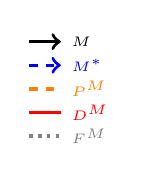
\begin{tikzpicture}[
very thick, 
->, 
every pin edge/.style={
	-, 
	very thin,
	decorate,
	decoration={snake},
	black!60,
}]
% \draw [help lines] (0,0) grid (3,2);

\tikzset{
	opt/.style={blue, dashed},
	d/.style={red, -},
	p/.style={orange, dashed,-},
	f/.style={gray, dotted,-},
}

\draw[] (3,1.3) -- (3.4,1.3) node[right]{\tiny $M$};
\draw[opt] (3,1) -- (3.4,1) node[right]{\tiny $M^*$};
\draw[p] (3,.7) -- (3.4,.7) node[right]{\tiny $P^M$};
\draw[d] (3,.4) -- (3.4,.4) node[right]{\tiny $D^M$};
\draw[f] (3,.1) -- (3.4,.1) node[right]{\tiny $F^M$};

% \graph[default graph]{
% 	{[nodes={d}]	3[x=0,y=0, pin=above right:{\small 2\$}],7[pin=below right:{\small 2\$}]};
% 	{[nodes={p}]	1[pin=above left:{\small 1\$}],2[pin=right:{\small 1\$}],4[pin=left:{\small 1\$}],5[pin=right:{\small 1\$}]};
% 	{[nodes={f}]	8,9,10};
% 	
% 	{1, 2} -> 3;
% 	{4, 5} -> 7;
% 
% 	{[edges={opt}]
% 	{1} -> 4;
% 	{8,9} -> 7;
% 	{2,3,10} -> 5;
% 	}
% };

\end{tikzpicture}
\end{figure}


To conclude this section, we show that our analysis is tight.
Consider the example given in Figure~\ref{fig:localtight}.
Assume, in this example, that there are no capacity constraints,
if the local search algorithm start by choosing vertex $3$ to be a driver, 
then the returned matching is the single edge $(2,3)$.
At this point, no further improvement can be done.
The optimal matching, on the other hand, is $\{(1, 2), (3, 2)\}$. 
The path in the example can be duplicated to form an arbitrary large graph (forest).

\begin{figure} 
\centering
\begin{tikzpicture}[every node/.style={draw, circle}]

\node[default node](a) at (0,0) {$1$};
\node[default node](b) at (2,0) {$2$};
\node[default node](c) at (4,0) {$3$};

\draw[->, dashed] (a) -- (b);
\draw[<->](b) -- (c);

\end{tikzpicture}

\caption{
\label{fig:localtight}
Local Search - Worst Case Example
}
\end{figure}